%-*- program: xelatex -*-        
%-*- program: biber -*-`        
%-*- program: xelatex -*-
\documentclass[11pt]{article}
\usepackage[margin=0.75in]{geometry}            % See geometry.pdf to learn the layout options. There are lots.
\geometry{letterpaper}  
\usepackage{amsmath,textcomp,amssymb,geometry,graphicx,enumerate,upquote,color}
\usepackage{hyperref}
\usepackage{breqn}
\usepackage{float}
\usepackage{tikz}
\usepackage{array}
\usepackage{float}
\usepackage{amsfonts}
\def\Session{Fall 2015}
\usepackage[english]{babel}
\title{Drawdown Project - Simulation}
\author{Boying Gong, Xinyue Zhou}
\newenvironment{qparts}{\begin{enumerate}[{(}a{)}]}{\end{enumerate}}
\def\endproofmark{$\Box$}
\newenvironment{proof}{\par{\bf Proof}:}{\endproofmark\smallskip}
\begin{document}
\maketitle

\tableofcontents

\clearpage

\section{Noice term with normal distribution}

To better understand the behaviour of conditional expected drawdown (CED) and the maximum drawdown distribution, we use some simple assumptions and paramters in this section as follows:

\begin{enumerate}
\item Noice term in the time series model follows Normal distribution with standard deviation of 0.01: $\epsilon \sim N(0, 0.0001)$.
\item Risk measures including volatility, VaR, ES and maximum drawdown are calculated based on simulated time series with path length 1000. The calculation of maximum drawdown is replicated 1000 times in order to obtain the maximum drawdown distribution and its tail mean (CED).
\item All time series parameters in this section range from -0.9 to 0.9. For time series with multiple parameters such as AR(2), ARMA(1, 1), the parameters are cartesian product of arithmetic progressions range from -0.9 to 0.9. Note that to take the stationary of AR and ARMA models into consideration (all moving averages are stationary, but the AR and ARMA model have to meet certain criteria), not all parameters in the cartesian product are used in the simulation.
\end{enumerate}

%%%%%%%%%%%%
\subsection{AR(1)} %%%%
%%%%%%%%%%%%

We started from the simplest model AR(1):

\begin{equation}
X_t = \kappa_1X_{t-1} + \epsilon_t
\end{equation}

We simulate AR(1) for various values of the autoregressive parameter for $\kappa_1 \in (-1, 1)$ . Figure \ref{fig:AR1_risk_measures} shows the relationship between AR(1) coefficient and risk measures of interest including ES, VaR, volatility and CED. Note that for AR(1) model, the order one serial correlation is the the value of autoregressive parameter.

CED shows a decreasing trend when $\kappa_1\in(-1, -0.75)$ and an increasing trend when $\kappa_1 \in(-0.75, 1)$. As shown in Figure \ref{fig:AR1_risk_measures}, it becomes feasible for us to distinguish negative and positive serial correlation using the CED values. However, the other 3 risk measures are all symmetric about $\kappa_1 = 0$, and they increase as the absolute values of $\kappa_1$ increases.

For VaR, ES and CED, the derivative of risk measure values to $\kappa_1$ approaches to zero as  $\kappa_1$ goes to 0 and increase as $\kappa_1$ increase. The trend of derivatives reverse for CED. While the change of $\kappa_1$ has a comparatively larger influence around 0, the influence becomes weaker as we move to larger  $\kappa_1$ values.

\begin{figure}[H]
\centering
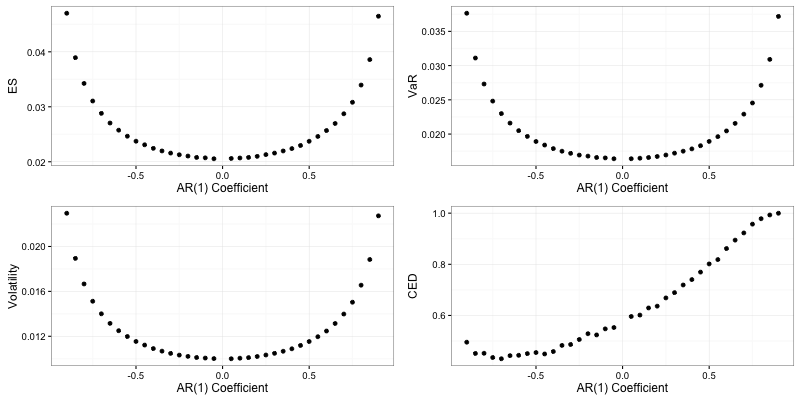
\includegraphics[width = 0.8\textwidth]{../figures/simulation/AR1_risk_measures}
\caption{AR(1): Relationship between auto-correlation coefficients and risk measures}
(Simulation path length: 1000, $\epsilon_t \sim N(0, 0.0001)$)
\label{fig:AR1_risk_measures}
\end{figure}

Figure \ref{fig:AR1_maxDrawdown_dist} shows the maximum drawdown distribution  Same as revealed in \ref{fig:AR1_risk_measures}, the mean and tail mean of maximum drawdown distribution increases as we increase $\kappa_1$ from negative values to positive values.

\begin{figure}[H]
\centering
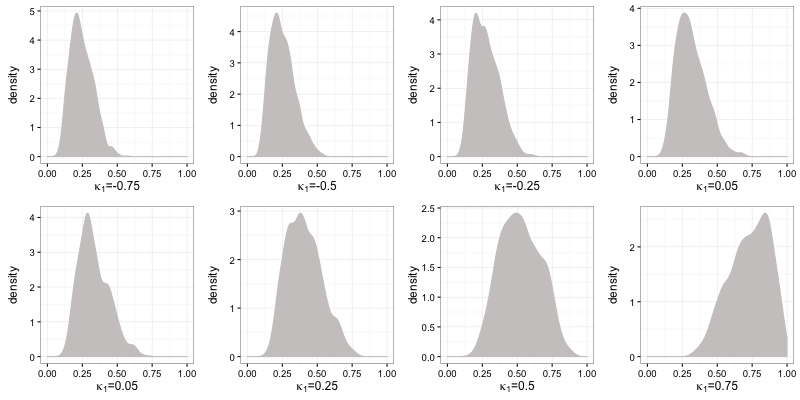
\includegraphics[width = 0.8\textwidth]{../figures/simulation/AR1_maxDrawdown_dist}
\caption{AR(1): Maximum drawdown distribution for various $\kappa_1$ values }
(Empirical distribution, path length = 1000, sample size = 1000, $\epsilon_t \sim N(0, 0.0001)$ )
\label{fig:AR1_maxDrawdown_dist}
\end{figure}

%%%%%%%%%%%%
\subsection{AR(2)} %%%%
%%%%%%%%%%%%

We then move to model AR(2):

\begin{equation}
X_t = \kappa_1X_{t-1} + \kappa_2X_{t-2}  + \epsilon_t
\end{equation}

Figure \ref{fig:AR2_risk_measures_pos} and \ref{fig:AR2_risk_measures_neg} shows the relationship between order one serial correlation and various risk measures.

\begin{figure}[H]
\centering
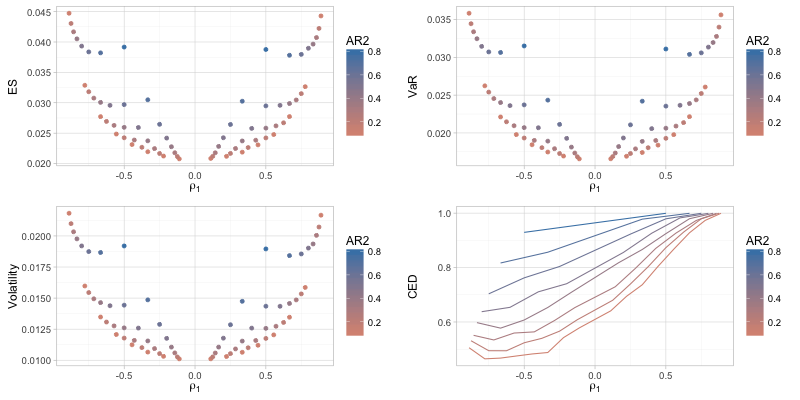
\includegraphics[width = 0.8\textwidth]{../figures/simulation/AR2_risk_measures_pos}
\caption{AR(2): Relationship between serial correlation $\rho_1$ and risk measures ($\kappa_2 > 0$)}
(Simulation path length: 1000, $\epsilon_t \sim N(0, 0.0001)$)
\label{fig:AR2_risk_measures_pos}
\end{figure}

\begin{figure}[H]
\centering
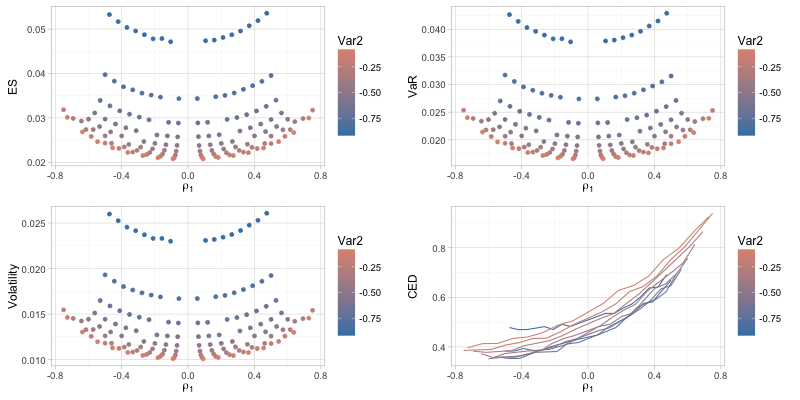
\includegraphics[width = 0.8\textwidth]{../figures/simulation/AR2_risk_measures_neg}
\caption{AR(2): Relationship between serial correlation $\rho_1$ and risk measures ($\kappa_2 < 0$)}
(Simulation path length: 1000, $\epsilon_t \sim N(0, 0.0001)$)
\label{fig:AR2_risk_measures_neg}
\end{figure}

\begin{figure}[H]
\centering
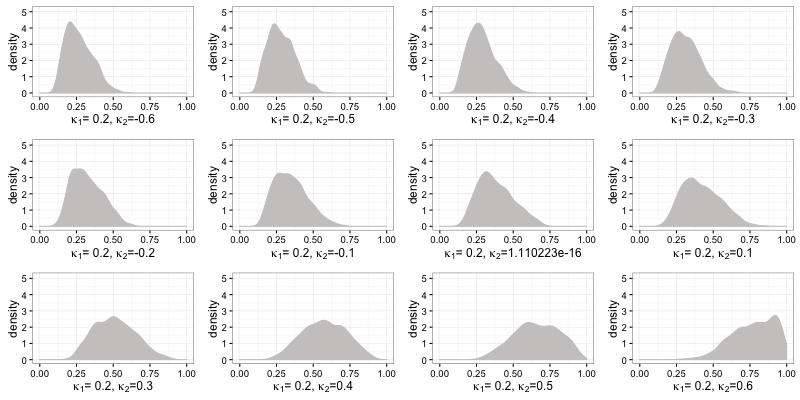
\includegraphics[width = 0.8\textwidth]{../figures/simulation/AR2_maxDrawdown_dist_kappa1_02}
\caption{AR(2): Maximum drawdown distribution for $\kappa_1 = 0.2$}
(Empirical distribution, path length = 1000, sample size = 1000, $\epsilon_t \sim N(0, 0.0001)$ )
\label{fig:AR2_maxDrawdown_dist_kappa1_02}
\end{figure}

\begin{figure}[H]
\centering
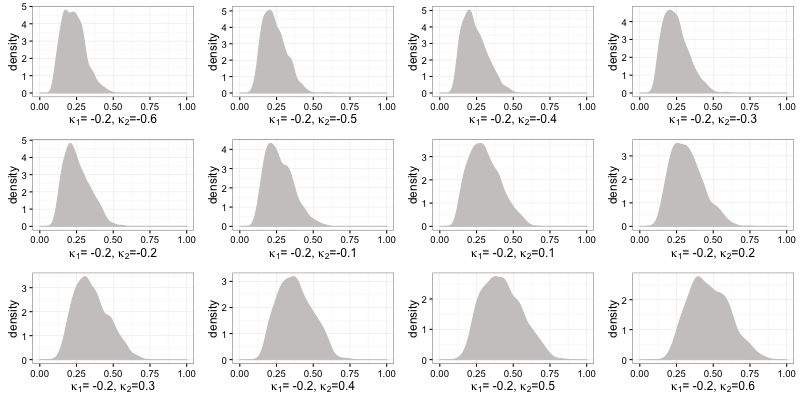
\includegraphics[width = 0.8\textwidth]{../figures/simulation/AR2_maxDrawdown_dist_kappa1_-02}
\caption{AR(2): Maximum drawdown distribution for $\kappa_1 = -0.2$}
(Empirical distribution, path length = 1000, sample size = 1000, $\epsilon_t \sim N(0, 0.0001)$ )
\label{fig:AR2_maxDrawdown_dist_kappa1_-02}
\end{figure}

%%%%%%%%%%%%
\subsection{MA(1)} %%%%
%%%%%%%%%%%%

\begin{equation}
X_t = \epsilon_t + \theta_1\epsilon_{t-1}
\end{equation}

\begin{figure}[H]
\centering
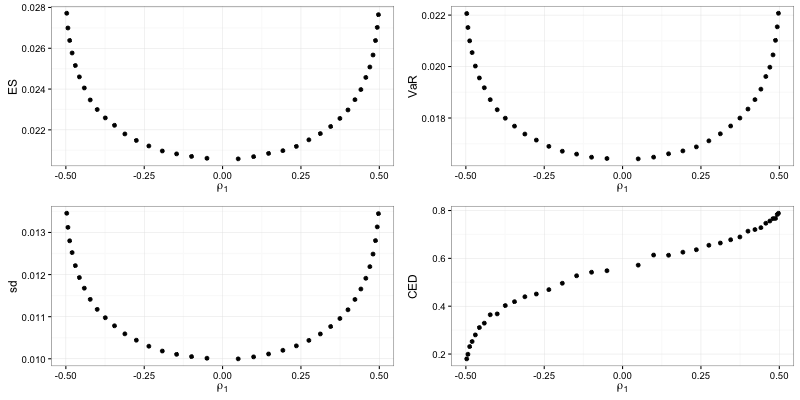
\includegraphics[width = 0.8\textwidth]{../figures/simulation/MA1_risk_measures_acf1}
\caption{MA(1): Relationship between serial correlation $\rho_1$ and risk measures}
(Simulation path length: 1000, $\epsilon_t \sim N(0, 0.0001)$)
\label{fig:MA1_risk_measures_acf1}
\end{figure}

\begin{figure}[H]
\centering
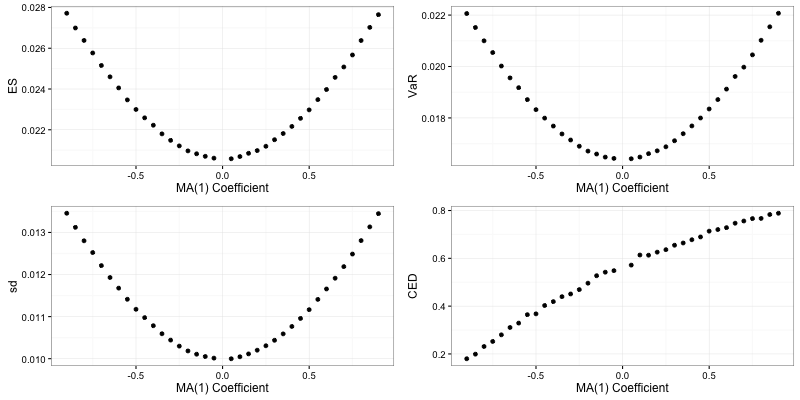
\includegraphics[width = 0.8\textwidth]{../figures/simulation/MA1_risk_measures_coefficient}
\caption{MA(1): Relationship between model coefficient and risk measures}
(Simulation path length: 1000, $\epsilon_t \sim N(0, 0.0001)$)
\label{fig:MA1_risk_measures_coefficient}
\end{figure} 

\begin{figure}[H]
\centering
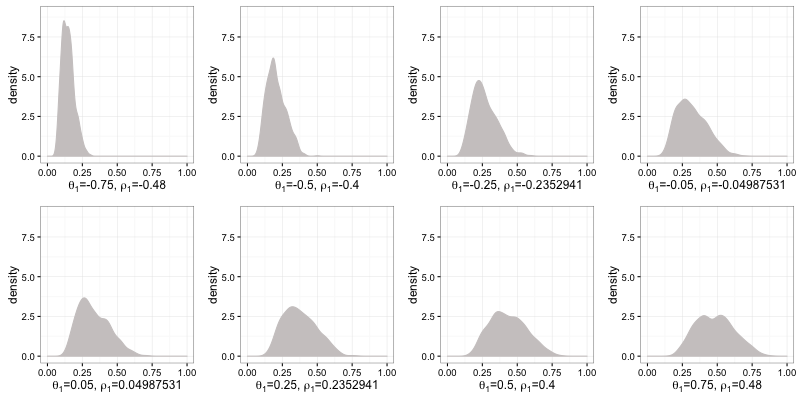
\includegraphics[width = 0.8\textwidth]{../figures/simulation/MA1_maxDrawdown_dist}
\caption{MA(1): Maximum drawdown distribution for various $\theta_1$ values}
(Empirical distribution, path length = 1000, sample size = 1000, $\epsilon_t \sim N(0, 0.0001)$ )
\label{fig:MA1_maxDrawdown_dist}
\end{figure}

%%%%%%%%%%%%
\subsection{MA(2)} %%%%
%%%%%%%%%%%%

\begin{equation}
X_t = \epsilon_t + \theta_1\epsilon_{t-1} + \theta_2\epsilon_{t-2}
\end{equation}

\begin{figure}[H]
\centering
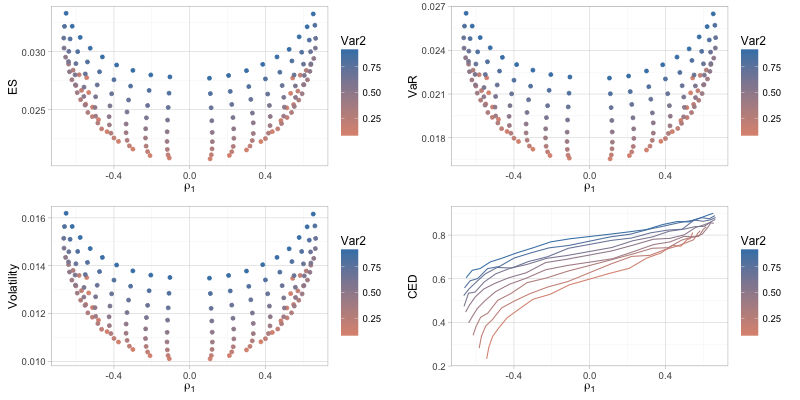
\includegraphics[width = 0.8\textwidth]{../figures/simulation/MA2_risk_measures_pos}
\caption{MA(2): Relationship between serial correlation $\rho_1$ and risk measures ($\theta_2>0$)}
(Simulation path length: 1000, $\epsilon_t \sim N(0, 0.0001)$)
\label{fig:MA2_risk_measures_pos}
\end{figure}

\begin{figure}[H]
\centering
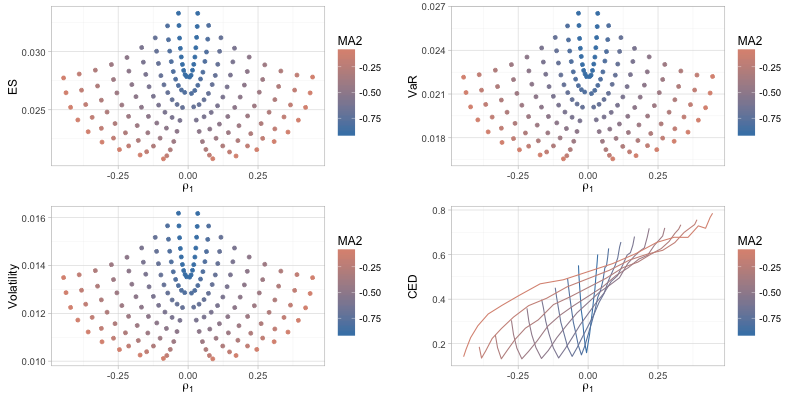
\includegraphics[width = 0.8\textwidth]{../figures/simulation/MA2_risk_measures_neg}
\caption{MA(2): Relationship between serial correlation $\rho_1$ and risk measures ($\theta_2<0$)}
(Simulation path length: 1000, $\epsilon_t \sim N(0, 0.0001)$)
\label{fig:MA2_risk_measures_neg}
\end{figure}

\begin{figure}[H]
\centering
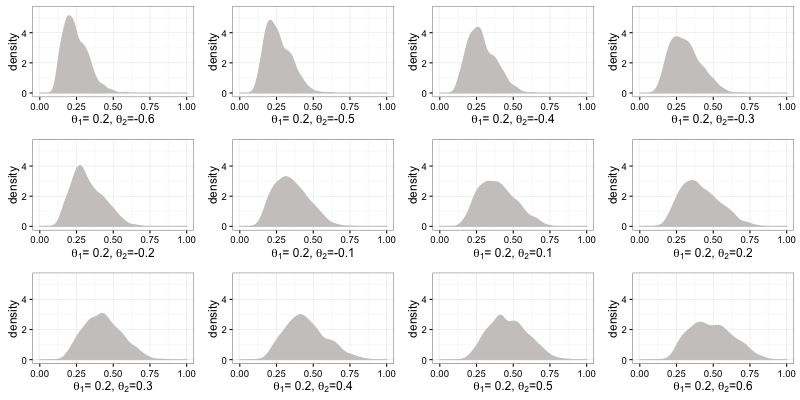
\includegraphics[width = 0.8\textwidth]{../figures/simulation/MA2_maxDrawdown_dist_theta1_02}
\caption{MA(2): Maximum drawdown distribution for $\theta_1 = 0.2$}
(Empirical distribution, path length = 1000, sample size = 1000, $\epsilon_t \sim N(0, 0.0001)$ )
\label{fig:MA2_maxDrawdown_dist_theta1_02}
\end{figure}

\begin{figure}[H]
\centering
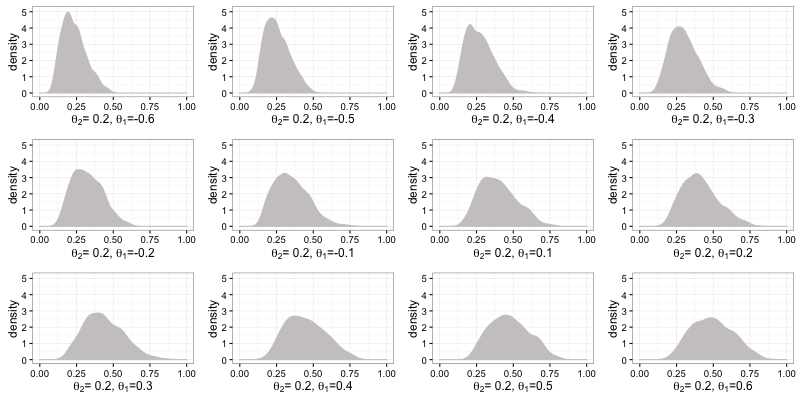
\includegraphics[width = 0.8\textwidth]{../figures/simulation/MA2_maxDrawdown_dist_theta2_02}
\caption{MA(2): Maximum drawdown distribution for $\theta_2 = 0.2$}
(Empirical distribution, path length = 1000, sample size = 1000, $\epsilon_t \sim N(0, 0.0001)$ )
\label{fig:MA2_maxDrawdown_dist_theta2_02}
\end{figure}


%%%%%%%%%%%%%%%%%%%%%%%%%
\subsection{ARMA(1, 1)} %%%%
%%%%%%%%%%%%%%%%%%%%%%%%%

\begin{equation}
X_t = X_{t-1} + \epsilon_t + \theta_1\epsilon_{t-1}
\end{equation}

\begin{figure}[H]
\centering
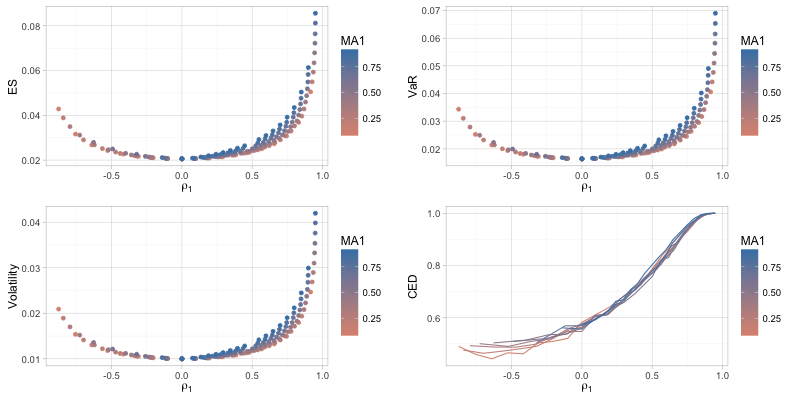
\includegraphics[width = 0.8\textwidth]{../figures/simulation/AR1MA1_risk_measures_pos}
\caption{ARMA(1, 1): Relationship between serial correlation $\rho_1$ and risk measures ($\theta_1>0$)}
(Simulation path length: 1000, $\epsilon_t \sim N(0, 0.0001)$)
\label{fig:AR1MA1_risk_measures_pos}
\end{figure}


\begin{figure}[H]
\centering
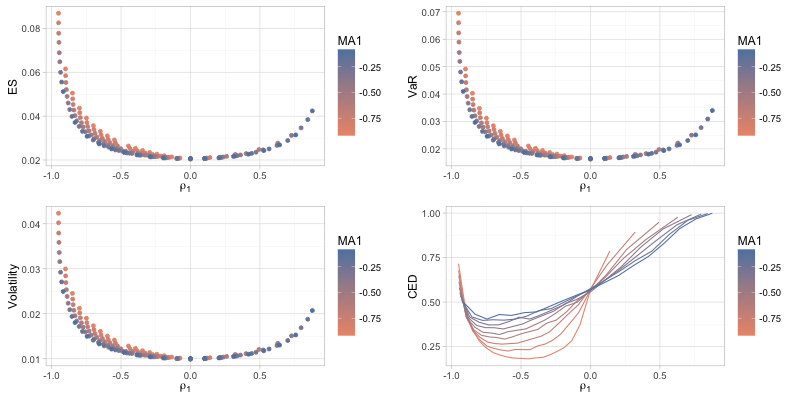
\includegraphics[width = 0.8\textwidth]{../figures/simulation/AR1MA1_risk_measures_neg}
\caption{ARMA(1, 1): Relationship between serial correlation $\rho_1$ and risk measures ($\theta_1>0$)}
(Simulation path length: 1000, $\epsilon_t \sim N(0, 0.0001)$)
\label{fig:AR1MA1_risk_measures_neg}
\end{figure}



%%%%%%%%%%%%%%%%%%%%%%%%%%%%%%%%%%%%%%%%%%%%%%%%%%
%%%%%%%%%%%%%%%%%%%%%%%%%%%%%%%%%%%%%%%%%%%%%%%%%%

\section{Noice term with student t distribution}

In this section, parameters used are close to what we've encountered in the empirical studies. 
\begin{enumerate}
\item White noice terms are simulated using t-distribution (degree of freedom = 4).
\item Set path length to 63, which is the number of trading days in three month.
\item Time series parameters all range from -0.3 to 0.3, which is similar to the financial time series data in the real world.
\end{enumerate}



\subsection{AR(1)}


\begin{figure}[H]
\centering
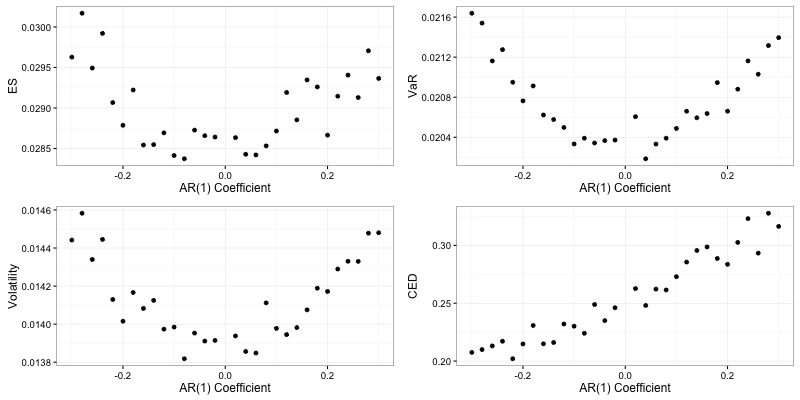
\includegraphics[width = 0.8\textwidth]{../figures/simulation/T_dist_AR1_risk_measures}
\caption{AR(1): Relationship between auto-correlation coefficients and risk measures}
(Simulation path length: 63, $\epsilon_t \sim 0.01T(df = 4)$)
\label{fig:T_dist_AR1_risk_measures}
\end{figure}



\begin{figure}[H]
\centering
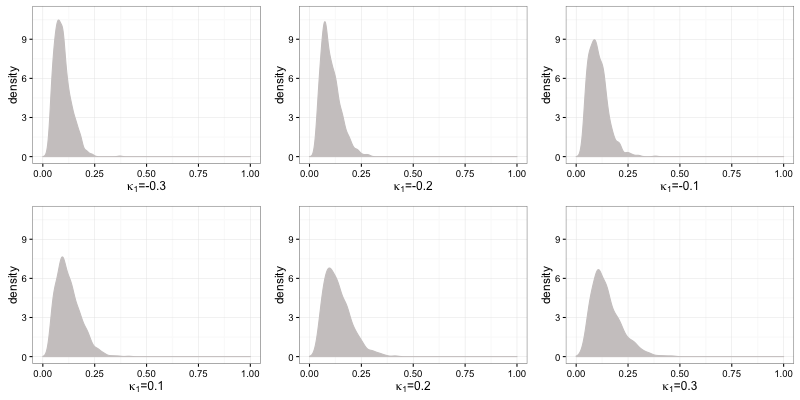
\includegraphics[width = 0.8\textwidth]{../figures/simulation/T_dist_AR1_maxDrawdown_dist}
\caption{AR(1): Maximum drawdown distribution for various $\kappa_1$ values }
(Empirical distribution, path length = 63, sample size = 1000, $\epsilon_t \sim 0.01T(df = 4)$)
\label{fig:T_dist_AR1_maxDrawdown_dist}
\end{figure}

\subsection{AR(2)}

\begin{figure}[H]
\centering
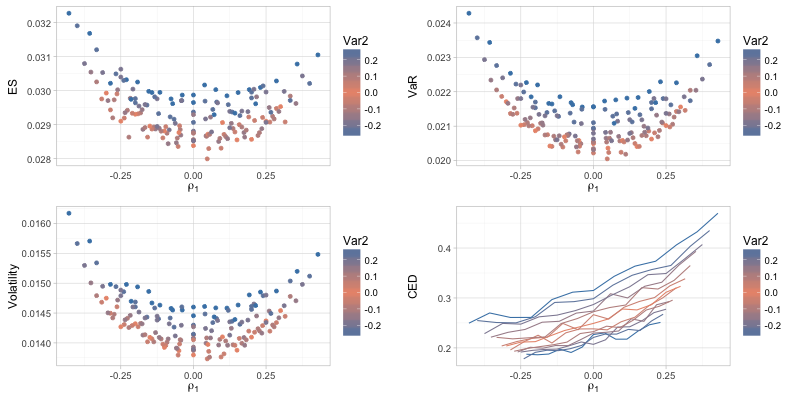
\includegraphics[width = 0.8\textwidth]{../figures/simulation/T_dist_AR2_risk_measures}
\caption{AR(2): Relationship between auto-correlation coefficients and risk measures}
(Simulation path length: 63, $\epsilon_t \sim 0.01T(df = 4)$)
\label{fig:T_dist_AR2_risk_measures}
\end{figure}

\begin{figure}[H]
\centering
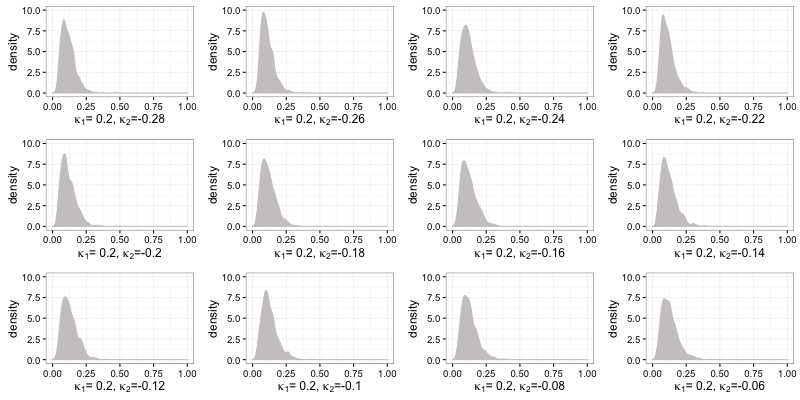
\includegraphics[width = 0.8\textwidth]{../figures/simulation/T_dist_AR2_maxDrawdown_dist_kappa1_02}
\caption{AR(2): Maximum drawdown distribution for various $\kappa_1$ values }
(Empirical distribution, path length = 63, sample size = 1000, $\epsilon_t \sim 0.01T(df = 4)$)
\label{fig:T_dist_AR2_maxDrawdown_dist_kappa1_02}
\end{figure}

\section{MA(1)}


\begin{figure}[H]
\centering
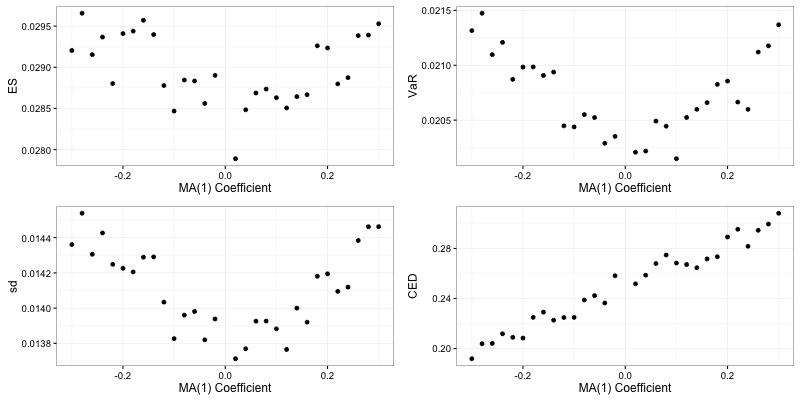
\includegraphics[width = 0.8\textwidth]{../figures/simulation/T_dist_MA1_risk_measures_coefficient.png}
\caption{MA(1): Relationship between serial correlation $\rho_1$ and risk measures}
(Simulation path length: 63, $\epsilon_t \sim 0.01T(df = 4)$)
\label{fig:T_dist_MA1_risk_measures_coefficient}
\end{figure}

\begin{figure}[H]
\centering
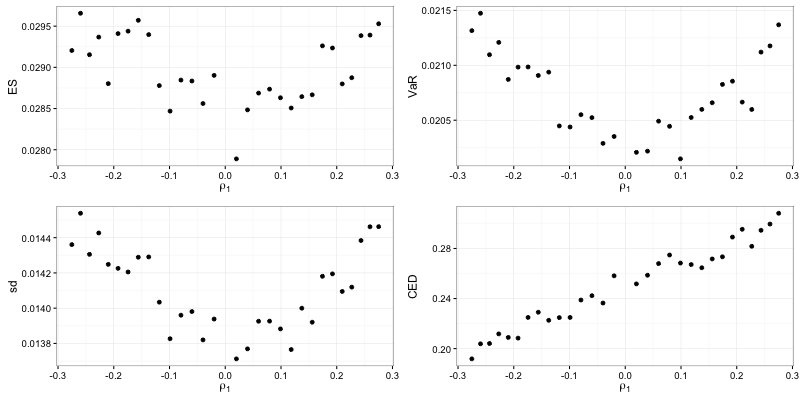
\includegraphics[width = 0.8\textwidth]{../figures/simulation/T_dist_MA1_risk_measures_acf1.png}
\caption{MA(1): Relationship between model coefficient and risk measures}
(Simulation path length: 63, $\epsilon_t \sim 0.01T(df = 4)$)
\label{fig:T_dist_MA1_risk_measures_acf1}
\end{figure} 

\begin{figure}[H]
\centering
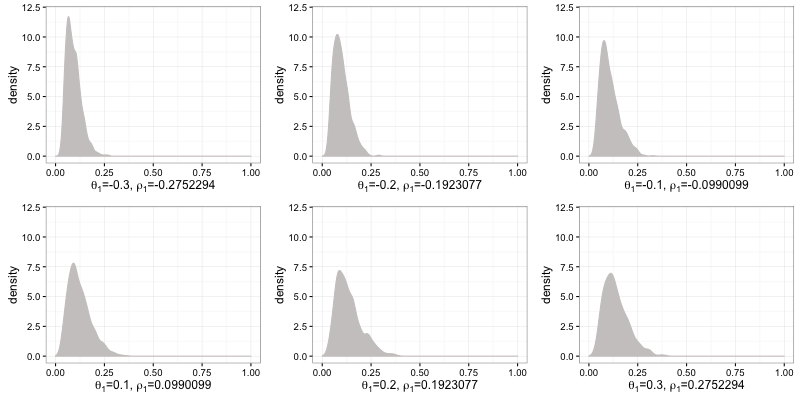
\includegraphics[width = 0.8\textwidth]{../figures/simulation/T_dist_MA1_maxDrawdown_dist}
\caption{MA(1): Maximum drawdown distribution for various $\kappa_1$ values }
(Empirical distribution, path length = 63, sample size = 1000, $\epsilon_t \sim 0.01T(df = 4)$)
\label{fig:T_dist_MA1_maxDrawdown_dist}
\end{figure}

\section{MA(1)}





T_dist_MA1_maxDrawdown_dist.png

%%%%%%%%%%%%%%%%%%%%%%%%%
\section{Thoughts}  %%%%%
%%%%%%%%%%%%%%%%%%%%%%%%%

The relationship between serial correlation are complicated even for simple models such as AR(2), MA(2) and ARMA(1, 1). We tried several ways to present the relationship. Plots in this report are the best we came up with.

We did not move to more sophisticated time series models with higher orders. The patterns in some sense explained why we hardly get informative relationship in our empirical data analysis. Real word data sets are usually more complex than simulation.

Usually financial data does not present strong serial correlation. If we could narrow down our scope to smaller serial correlations we may found that the serial correlation is more closely realted with vaious risk measures.

Further efforts:
Add Garch model 
Change the white noice term from normal distribution to more heavy tailed distribution such as student-t distribution.


\end{document}
